\section{Krypto}
\label{Krypto}
Die Krypto-Architektur ergibt sich aus der Anforderung Bitcoin-Transaktionen automatisiert durchführen zu können und gleichzeitig ein hohes Sicherheitsniveau sicherzustellen. 
Die besondere Schwierigkeit besteht darin, dass das Hot-Wallet direkt auf das Internet zugreifen können muss und dementsprechend als internet-exponiertes System einem erhöhten Risiko ausgesetzt ist.
Dieses gilt es ausreichend vor Kompromittierung zu schützen da bei eben diesem Fall potenziell unmittelbar auf kryptographische Schlüssel zugegriffen werden könnte und der Wallet-Inhalt transferiert werden könnte.
In Zuge dessen wird es ebenfalls von den obig beschriebenen Services vor aus dem Gefahrmodell bekannten Angriffen geschützt und erweist so bereits eine erhöhte technische Sicherheit auf.
Um diesen Gedanken fortzuführen wurde sich für eine besonders sichere Konzeptionelle und Architektonische Ausarbeitung entschieden. Dementsprechend wurde ein Hot-/Cold-Wallet-Architekturmodell gewählt, wie es im institutionellen und betrieblichen Umfeld als Best Practice eingesetzt wird \cite{knowingbitcoin_hotcold, nadcab_custodial_arch, riskpublishing_hotcold}. Dieses Modell kombiniert operative Verfügbarkeit mit Schlüsseltrennung und stellt die nötige Sicherheitsfunktion zur Anforderung des Mandanten dar.

\subsection{Hot- und Cold-Wallet Architektur}

Im Sinne einer klassischen Hot- und Cold-Wallet-Architektur hält das Hot-Wallet lediglich einen begrenzten Anteil der monetären Mittel (ca.\ 5\,\%) \cite{nadcab_custodial_arch, riskpublishing_hotcold}, während der überwiegende Teil der Assets im Cold-Wallet verwahrt wird. Dieses Modell reduziert den potenziellen Schaden bei einer Kompromittierung des Online-Systems erheblich, da nur ein kleiner Teil der monetären Mittel extrahiert werden kann.

Während das Hot-Wallet für automatisierte Transaktionen genutzt wird, erfolgen Transfers aus dem Cold-Wallet ausschließlich kontrolliert und mit manueller Freigabe. Insbesondere Cold-to-Hot-Transfers werden bewusst nicht vollautomatisiert, da sie größere Wertbeträge betreffen \cite{knowingbitcoin_hotcold Wallets, Hot_VS_Cold-Wallet, psbt_dcentral}.

\subsection{Hot-Wallet}

Da die Hot-Wallet dauerhaft mit dem Internet verbunden ist, stellt sie die am stärksten exponierte Komponente der Architektur dar. Entsprechend wird dieses System besonders gehärtet und folgt strikt dem Prinzip der \emph{Segregation of Duties}. Ziel ist es, zu verhindern, dass ein einzelner Dienst Transaktionen eigenständig aufbauen, autorisieren und signieren kann \cite{nadcab_custodial_arch}.

\subsubsection{Bitcoin Core Node}

Bitcoin Core wird ausschließlich als Full Node ohne aktivierte Wallet-Funktion betrieben. Die Node übernimmt die Validierung von Blöcken und Transaktionen, Mempool-Verwaltung sowie Gebührenschätzungen, besitzt jedoch keine kryptographischen Schlüssel \cite{bitcoin_core_arch, bitcoin_core_docs, Sparrow_Wallets_Node_Connect}.  

Durch die Trennung von Node- und Wallet-Funktionalität wird verhindert, dass ein Angreifer nach einer Kompromittierung der Node Transaktionen direkt signieren und veröffentlichen kann.

\subsubsection{Transaktionsaufbau und Orchestrierung}

Der Transaktionsaufbau erfolgt in einer dedizierten Orchestrierungs- und Middleware-Komponente. Diese überwacht den Wallet-Zustand, evaluiert definierte Thresholds und erstellt auf dieser Basis Transaktionsentwürfe (PSBTs oder Raw-TXs).  
Sicherheitsrelevante Entscheidungen trifft diese Komponente nicht selbst, sondern übergibt Transaktions-Intents an eine dedizierte Policy-Instanz.

\subsubsection{Open Policy Agent}

Die autorisierende Entscheidung über Transaktionen erfolgt zentral über den Open Policy Agent (OPA). OPA evaluiert Transaktionsanfragen anhand konfigurierbarer Regeln wie Betragslimits, Whitelists, Zeitfenstern oder Velocity-Checks. Die Policy-Logik ist dabei vollständig von der Applikationslogik entkoppelt und ist frei wählbar \cite{opa_docs, opa_microservices}.  

OPA übernimmt die Policy‑Entscheidung, während die Middleware als Enforcement Point die Ausführung strikt an das Ergebnis koppelt; Policy‑Entscheidungen werden revisionsfähig protokolliert und in die Postgres-Datenbank geschrieben.

Diese Trennung erhöht die Wartbarkeit, Revisionssicherheit und Nachvollziehbarkeit sicherheitskritischer Entscheidungen.

Folgende OPA Policies wurden im Zuge der System-operationalisierung erstellt, können jedoch anhand des use cases des Mandanten angepasst werden
=====================================
GUI script hierfür????
OPA Playground?

\subsubsection{Signer-Instanz}

Die Signer-Instanz stellt eine eigene Sicherheitsdomäne dar und hält keine Bitcoin-Private-Keys. Stattdessen erzeugt sie kryptographisch signierte Freigaben für Transaktionen.  
Jede Freigabe ist eindeutig an den Hash der zugehörigen PSBT gebunden und dient als formaler Autorisierungsnachweis für die nachfolgenden Signaturschritte im Cold-Bereich.

\subsubsection{Monitoring}

Ein zentrales Monitoring überwacht den vollständigen Transaktions-Lifecycle sowie den Zustand der Hot-Wallet. Erfasst werden unter anderem Wallet-Balance, ausstehende Transaktionen und definierte Sicherheits-Thresholds.  
Auffälligkeiten oder Grenzwertverletzungen werden automatisiert gemeldet und ermöglichen eine schnelle operationelle Reaktion.

Ebenfalls wird sparrow als watch-only GUI im server modus integriert, um einem menschlichen Operanden das Verfolgen der Transaktionen und Wertgegenstände zu ermöglichen. \cite{Sparrow_Wallets_Features}

\subsubsection{Key Holder???}
key holder ist der policy signer mit dem speicherort im kubernetes secrets

AWS KMS hinzufügen?

\subsection{Cold-Wallet}

\subsubsection{Architektur}

Das Cold-Wallet ist vollständig air-gapped und besitzt keinerlei Netzwerkverbindung. Die Systeme werden auf dedizierten virtuellen Maschinen in der proxmox Umgebung betrieben, deren Netzwerkfunktionen sowohl auf Betriebssystem- als auch auf Hypervisor-Ebene deaktiviert sind \cite{airgap_psbt_guide, Wallets}.

Das vom Internet isolierte Cold-Wallet bildet den architektionischen Kern des Systems und verwaltet (ca.\ 95\,\%), der Bitcoins. Diese gilt es dementsprechend besonders zu schützen, weshalb sich für ein air-gap und ein 2 aus 3 Multi-Signatur Wallet entschieden wurde. Die Isolierung des Systems reduziert die Angriffsfläche gegenüber netzwerkbasierten Angriffen erheblich und verhindert direkte Remote-Kompromittierungen.

Unter der Voraussetzung eines sicheren Perimeters am Standort des Mandanten verbleibt somit nur eine Bedrohung des operationellen Prozesses im Signierungs-Prozess. Um diesen sicher zu gestalten wurde sich für ein 2 aus 3 Multi-Signatur Prozess entschieden, wobei über einen USB stick partially signed bitcoin transactions (PSBTs) transferiert werden können.\cite{riskpublishing_hotcold, bip174, Sparrow_Wallets_Best_Practices, knowingbitcoin_hotcold, psbt_dcentral, airgap_psbt_guide}.
Dieser Multi-signature Prozess wird besonders für hohe Geldsummen und professionelle Architekturen empfohlen und findet dementsprechend Verwendung \cite{Sparrow_Wallets_Best_Practices}.

Als Betriebssystem kommt NixOS zum Einsatz, um reproduzierbare, direkt dokumentierte und minimalistische Konfigurationen zu gewährleisten. Sparrow Wallet fungiert entweder als Multisig-Koordinator und PSBT-Handler oder als key Holder. Eine Instanz hält nicht beide Rollen gleichzeitig, wodurch ein kompromittiertes System nicht Koordinations- als auch Signierungsschritte gleichzeitig durchführen kann.  \cite{nixos_funktionsweise, sparrow_docs, sparrow_multisig}.

Das Cold-Wallet besteht aus drei separaten virtuellen Maschinen: zwei Key-Holder-Instanzen (Key B und Key C) sowie einer Koordinator-Instanz. Das Multisignature-Wallet ist als 2-aus-3-Modell konfiguriert.

Der Schlüssel des Hot-Wallets (Key A) ist integraler Bestandteil des operativen Prozesses. Transaktionen werden im Hot-System erzeugt und bereits initial mit Key A signiert. Die resultierende PSBT ist somit bei Eintritt in den Cold-Bereich bereits kryptographisch an den Hot-Wallet Schlüssel gebunden und kann darüber authentifiziert werden.

Die in BIP‑174 definierten Rollen (Creator, Updater, Signer) beschreiben logische Verarbeitungsschritte und nicht zwingend getrennte Akteure. Dabei wird explizit erwähnt, dass der Creator mit dem Updator und der Updator mit dem Signer zusammengelegt werden dürfen. Die Spezifikation erlaubt die Zusammenlegung mehrerer Rollen innerhalb derselben Instanz und wurde dementsprechend auf diese Weise implementiert. Die andere Rollen werden von je einer VM übernommen.
Die Spezifikation sowie Referenzimplementierungen wie Bitcoin Core sehen ausdrücklich vor, dass eine einzelne Instanz mehrere dieser Rollen gleichzeitig übernehmen kann. Entsprechend ist es zulässig, dass das Hot‑Wallet eine PSBT nicht nur erstellt, sondern diese auch unmittelbar teilweise signiert, bevor sie an weitere Signer übnergeben wird \cite{bip174}.

\begin{table}
\centering

\begin{tabular}{c c c}
\textbf{Key} & \textbf{Ort} & \textbf{Rolle} \\
\textbf{Key A} & Hot‑System & Operatives Signing \\
\textbf{Key B} & Cold‑VM (air‑gapped) & Sicherheitsanker \\
\textbf{Key C} & Cold‑VM (air‑gapped)& Recovery \\

\end{tabular}

\end{table}
Durch dieses Vorgehen kann die Authentizität der Transaktion bereits vor der Koordination im Cold-Wallet nachgewiesen werden und zeigt, dass diese nicht im Transit modifiziert wurde. Die nachgelagerten Cold-Signaturen durch Key\~B und Key\~C ergänzen diese initiale Signatur gemäß dem PSBT-Workflow \cite{bip174, sparrow_multisig}.

Wie bereits erwähnt kann neben der primär dargestellten Implementation der Mandant nach Übergabe des simulierten System entscheiden dediziert Hardware Wallets anstatt der Key-Holder NixOS VM zu verwenden.
Dementsprechend wäre das Aufsetzen von Schlüssel B und C abzuändern.

Zur Wiederherstellung werden Seeds der Offline‑Signer (KeyB/KeyC) sowie der Wallet‑Descriptor/Xpub‑Satz separat und redundant gesichert. Durch das 2‑aus‑3‑Multisig‑Modell bleibt die Spend‑Fähigkeit auch bei Ausfall eines einzelnen Keys erhalten.

\subsubsection{Rolle von Sparrow Wallet im Cold-Wallet}

Sparrow Wallet fungiert im Cold-Wallet ausschließlich als Multisignature-Koordinator und PSBT-Handler. Die Applikation verwaltet keine vollständige Blockchain und besitzt keine Netzwerkverbindung. Private Keys verbleiben ausschließlich auf den jeweiligen Cold-Key-Systemen.

Sparrow übernimmt im Cold-Bereich folgende Aufgaben:
\begin{itemize}
  \item Import und Anzeige freigegebener PSBTs,
  \item Koordination der Multisignature-Signaturen,
  \item Überprüfung der Skript- und Adressstruktur,
  \item Zusammenführung und Finalisierung der Signaturen.
\end{itemize}

Durch die ausschließliche Nutzung von PSBTs wird sichergestellt, dass sensitive Schlüsselmaterialien das air-gapped System niemals verlassen und keine Signaturschritte außerhalb der expliziten Benutzerinteraktion erfolgen.

Sparrow zeichnet sich zudem mit passenden Eigenschaften aus, wodurch es sich für das Aufesetzen von airgapped in unserer Architektur eignet. Unter diese Besonderheiten fallen die Möglichkeit des Einsaztes als Descriptor-Wallets, die Watch-Only-Konfigurationen sowie die native PSBT-Workflow Unterstützung. Insbesondere die transparente Darstellung von Inputs, Outputs, Gebühren und Signaturstatus ermöglicht eine nachvollziehbare manuelle Prüfung durch den Operator, weshalb es auch im Hot-Wallet zum Einsatz kommt. \cite{sparrow_multisig, sparrow_docs, Sparrow_Wallets_Features, airgap_psbt_guide}

Anzuführen ist ebenfalls, dass sparrow sich im Zuge der Implementierung durch einen Fehler im stable release auszeichnete. Nach dem Download aus dem Nix-Store und Ausführen des Programns ergaben sich Probleme mit der JavaFX Bibliothek und verschiedene Fenster mit dem Fehler \textbf{Panes omitted)} konnten nicht anzeigt werden.
Aufgrund dessen hatten wir uns bei sparrow für die unstable Version entschieden, die Java25 nativ unterstützt und diese Probleme behob.

\subsubsection{Sicherheitsmodell}

Das Cold-Wallet ist als 2-aus-3-Multisignature-Wallet implementiert. Die erforderlichen Private Keys befinden sich auf voneinander isolierten Systemen.  
Der Austausch von Transaktionsdaten erfolgt ausschließlich über PSBTs gemäß BIP-174, wodurch Private Keys das air-gapped System niemals verlassen \cite{bip174, psbt_dcentral, nist_zero_trust}.

\paragraph{Hash-basierte Transaktionsfreigabe (Approval Layer)}

Zusätzlich zur eigentlichen Bitcoin-Multisignature wird eine vorgeschaltete, hashbasierte Freigabeschicht eingesetzt. Diese dient nicht der Autorisierung von Bitcoin-Outputs und damit dem Schutz der Bitcoin-Assets selbst, sondern der Integrität des organisatorischen Freigabeprozesses einer Transaktion innerhalb des Systems. Dadurch kann auf Signer-VM kontrolliert werden, dass die Koordinator Instanz diese Transaktion freigegeben hat und sie nicht in-transit bearbeitet wurde.

Zur Härtung des USB Austausch Prozess wurde sich für einen zusätzliche Hash-Funktionalität als Sicherheitsanker entschieden. Damit kann sichergestellt werden, der USB nicht im transit ausgetauscht wurde und vom einen der autorisierten Systeme stammt. 
In Anwendungsfall des Mandanten wird das physische Umstecken des USB Sticks verlangt, wobei kein Austausch der PSBTs oder des USB möglich sein sollte. Nichtsdestotrotz wurde der menschliche Fehler wie Unterbrechen des Prozesses und eine Kompromittierung in dieser Pause eingeplant und wird durch diese Schicht unterbunden.
Der Mandant kann des USB Austausch ebenfalls durch die Generierung von QR-Codes und eine Kamera an den VMs oder durch direkte hardware Wallets ersetzen. Diese machen die zusätzliche Hash-kontrolle Überflüssig, da die direkte Erkennung des QR-Codes und PSBT Erkennung nicht-störbar sein sollte und die Hardware-Wallets solch eine Schicht oft direkt integrieren. \cite{Wallets, knowingbitcoin_airgap,Hardware_VS_Cold-Wallet}
Ein Aufsetzen solch einer hardware Wallet sollte im Zuge dieser Ausarbeitung nicht verwendet werden, da es die Aufgabe des Aufsetzen einer eigenen Architektur zu einem großen Teil aushebeln würde. Zudem konnte diese Technologie als auch die visuelle Übertragung per QR-Code und Kamera nicht in der proxmox-Labor Umgebung virtualisiert werden. Der USB-Austausch stellt sich als einfaches Wechseln des besitzer einer virtualisierten Festplatte dar und konnte somit sehr gut für die sptere praktische Verwendung simuliert werden.

Dabei kann über \texttt{scripts/auth/hash-keyGen.sh} ein Schlüsselpaar auf der Koordinator Instanz generiert werden und der public key auf einem USB gespeichert werden.
Dieser separate kryptographischen Schlüssel dient ausschließlich der Freigabe von psbt TX und soll deren Herkunft von den vetrauten Systemen verifizieren. Sie bestätigt, dass die PSBTs nicht im Transit kompromittiert wurden.
Der USB wird dann auf der key B und key C VM eingesteckt, explizit gemountet und über \texttt{scripts/auth/hash-keyStore.sh} der public Key extrahiert.
Als weitere Sicherheitsebene muss der Nutzer die Übereinstimmung Hex-Signatur bei Erstellung des Schlüsselpaars und beim Speichern des public key verifizieren.
Ohne dies könnte der public Key in transit ausgetauscht werden und die chain-of-trust wäre unterbrochen, was zur Verifizierung von nicht mit dem Koordinator abgestimmten TX genutzt werden könnte.

Key A benötigt diese zusätzliche Hash-Verifikation nicht, da die Transaktion bereits initial im Hot-System erzeugt und signiert wird. Die Authentizität der PSBT kann somit bereits vor Eintritt in den Cold-Bereich kryptographisch nachvollzogen werden.
Der spätere Broadcast im Hot-System stellt keinen sicherheitskritischen Schritt dar. Unvollständige oder manipulierte Transaktionen werden vom Bitcoin-Netzwerk abgewiesen, wodurch der Broadcast-Prozess keine zusätzliche Vertrauensannahme erfordert. Ein vollständiger Austausch der PSBTs vor broadcast mit einer anderen Funktionalen ist ebenfalls zu vernachlässigen, da diese nicht von der COld-Wallet signiert wurde und dementsprechend nicht deren bitcoins beeinflussen kann. Diese kann ohne Verlust von Assets gebroadcasted werden.Eine Kompromittierung dieses Schrittes hätte nur einen vorübergehenden Verlust des Schutzzieles der Verfügbarkeit zu Tragen. Dieser hätte zwar keinen Verlust an Assets zur Folge, gilt jedoch Nichtsdestotrotz zu vermeiden.

Das script \texttt{scripts/psbt/psbt-approve} kann auf der Koordinator VM ausgeführt werden und erstellt zusätzliche Artefakte als Sicherheitsebene, welche die Freigabe eindeutig an genau eine PSBT-Version bindet
Dieses enhält:
\begin{itemize}
  \item Metadaten zur Transaktion,
  \item eine eindeutige Transaktions-ID,
  \item einen kryptographischen Hash der zugehörigen PSBT.
\end{itemize}
  
Zudem können diese dann auf der Key-Holder VM über \texttt{scripts/auth/hash-verify.sh} auf Übereinstimmung mit dem auf der VM gespeicherten hash-Material überprüft werden.

Der xpub code zum Aufetzen der keyHolder Instanzen und der public Key für die hash Funktionalität können auf demselben USB-Stick zeitgleich transportiert werden und vereinfachen den Deployment-Prozess

Die zusätzliche Hash-Kontrolle entfällt als nicht-Umsetzbar und meist bereits integriert beim Wechsel von air-gapped VMs zu Hardware-krypto-Wallets.


\subsection{Schnittstelle und Workflow}

Der Datenaustausch zwischen Online- und Offline-Systemen erfolgt ausschließlich über ein dediziertes Wechselmedium. Pro Zeitpunkt befindet sich stets nur eine Transaktion auf dem Medium, wodurch Verwechslungen und Zustandsinkonsistenzen vermieden werden.

Der workflow-basierte Ablauf gestaltet sich wie folgt:
\begin{itemize}
  \item Erstellung einer PSBT im Hot-System
  \item Kryptographische Freigabe durch die Signer-Instanz
  \item Verifikation der Freigabe und Multisignature-Signatur im Cold-Wallet
  \item Zusammenführung und Finalisierung der Signaturen
  \item Broadcast der finalen Transaktion durch das Hot-System

\end{itemize}

Der Offline‑Workflow basiert auf PSBT gemäß BIP‑174, welches explizit Multi‑Signer- und Air‑gapped‑Signaturen unterstützt. \cite{bip174}

\begin{figure}
    \centering
    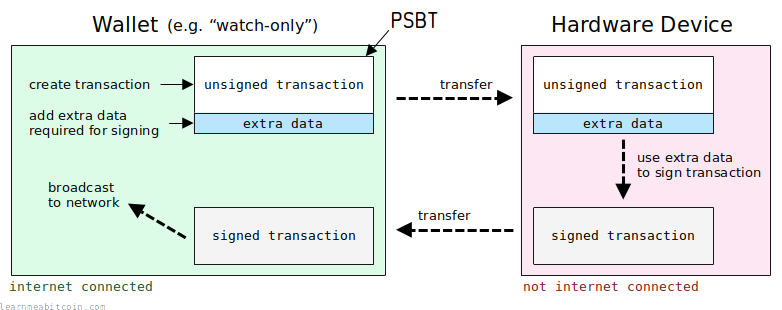
\includegraphics[width=0.5\linewidth]{image.png}
    \caption{Enter Caption}
    \label{fig:placeholder}
\end{figure}
https://learnmeabitcoin.com/technical/transaction/psbt/


Dieser Ansatz kombiniert automatisierte Abläufe mit gezielten manuellen Kontrollpunkten und stellt sicher, dass selbst bei einer vollständigen Kompromittierung des Online-Systems kein unautorisierter Zugriff auf die monetär größeren Cold-Assets möglich ist.


Aufgrund der vorhandenen Full-Node-Infrastruktur wird Sparrow Wallet direkt mit Bitcoin Core verbunden. Die Nutzung öffentlicher Electrum-Server entfällt, da diese zwar keine Gefährdung der Assets darstellen, jedoch Wallet-Metadaten gegenüber dem Serverbetreiber offenlegen können. Ein zusätzlicher privater Electrum-Server wurde aufgrund des erhöhten Betriebsaufwandes und des begrenzten Mehrwerts innerhalb des Projektumfangs nicht implementiert. \cite{sparrow_quick, Sparrow_Wallets_Node_Connect}